%You can leave alone everything before Line 79.
\documentclass{article}
\usepackage{url,amsfonts, amsmath, amssymb, amsthm,color, enumerate}
 \usepackage{fullpage}
% Page layout
%\setlength{\textheight}{8.75in}
%\setlength{\columnsep}{2.0pc}
%\setlength{\textwidth}{6.5in}
%\setlength{\topmargin}{0in}
%\setlength{\headheight}{0.0in}
%\setlength{\headsep}{0.0in}
%\setlength{\oddsidemargin}{0in}
%\setlength{\evensidemargin}{0in}
%\setlength{\parindent}{1pc}
\newcommand{\shortbar}{\begin{center}\rule{5ex}{0.1pt}\end{center}}
%\renewcommand{\baselinestretch}{1.1}
% Macros for course info
\newcommand{\courseNumber}{EECS 545}
\newcommand{\courseTitle}{Machine Learning}
\newcommand{\semester}{Winter 2012}
% Theorem-like structures are numbered within SECTION units
\theoremstyle{plain}
\newtheorem{theorem}{Theorem}[section]
\newtheorem{lemma}[theorem]{Lemma}
\newtheorem{corollary}[theorem]{Corollary}
\newtheorem{proposition}[theorem]{Proposition}
\newtheorem{statement}[theorem]{Statement}
\newtheorem{conjecture}[theorem]{Conjecture}
\newtheorem{fact}{Fact}
%definition style
\theoremstyle{definition}
\newtheorem{definition}[theorem]{Definition}
\newtheorem{example}{Example}
\newtheorem{problem}[theorem]{Problem}
\newtheorem{exercise}{Exercise}
\newtheorem{algorithm}{Algorithm}
%remark style
\theoremstyle{remark}
\newtheorem{remark}[theorem]{Remark}
\newtheorem{reduction}[theorem]{Reduction}
%\newtheorem{question}[theorem]{Question}
\newtheorem{question}{Question}
%\newtheorem{claim}[theorem]{Claim}
%
% Proof-making commands and environments
\newcommand{\beginproof}{\medskip\noindent{\bf Proof.~}}
\newcommand{\beginproofof}[1]{\medskip\noindent{\bf Proof of #1.~}}
\newcommand{\finishproof}{\hspace{0.2ex}\rule{1ex}{1ex}}
\newenvironment{solution}[1]{\medskip\noindent{\bf Problem #1.~}}{\shortbar}

%====header======
\newcommand{\solutions}[4]{
%\renewcommand{\thetheorem}{{#2}.\arabic{theorem}}
\vspace{-2ex}
\begin{center}
{\small  \courseNumber, \courseTitle
\hfill {\Large \bf {#1} }\\
\semester, University of Michigan, Ann Arbor \hfill
{\em Date: #3}}\\
\vspace{-1ex}
\hrulefill\\
\vspace{4ex}
{\normalsize Project Progress Report}\\
%{\LARGE  TITLE #2}\\
\vspace{2ex}
\end{center}
\begin{trivlist}
\item \textsc{Team members:} {#4}
\end{trivlist}
\noindent
\shortbar
\vspace{3ex}
}
% math macros
\newcommand{\defeq}{\stackrel{\textrm{def}}{=}}
\newcommand{\Prob}{\textrm{Prob}}
%==
\usepackage{graphicx}
\begin{document}
%%%%%%%%%%%%%%%%%%%%%%%%%%%%%%%%%%%%%%%%%%%%%%%%%
%\solutions{Your name}{Problem Set Number}{Date of preparation}{Collaborators}{Prover}{Verifiers}
\solutions{}{}{\today}{\\ Keegan R. Kinkade, @kinkadek\\ Pedro d'Aquino, @pdaquino \\Shiva Ghose, @gshiva }
%%%%%%%%%%%%%%%%%%%%%%%%%%%%%%%%%%%%%%%%%%%%%%%%%
%\renewcommand{\theproblem}{\arabic{problem}} 
%%%%%%%%%%%%%%%%%%%%%%%%%%%%%%%%%%%%%%%%%%%%%%%%%
%
% Begin the solution for each problem by
% \begin{solution}{Problem Number} and ends it with \end{solution}
%
% the solution for Problem 

\begin{abstract}

In order for artificial intelligence agents to autonomously operate within a given environment, they must be capable of processing perceptual knowledge in such a manner as to intelligently interact with their environment. For a competitively driven AI agent, this becomes increasingly important, as the inability to intelligently process perceptual information will ultimately lead to defeat by those who are capable of such computation. To this end, the following describes the implementation of sophisticated machine learning techniques in an artificially driven tank battle simulator. Armed with such techniques, it is the goal of this project to provide a competitive, autonomous AI agent with the ability to determine how to best evade an opponent's attacks while striking in such a manner as to maximize the possibility of destroying the enemy. 

\end{abstract}

\section{Introduction}

Initially released in 2001 with the aim of assisting in learning object oriented programming, Robocode is an open source tank battling simulator implemented in Java. Each Robocode agent is designed with the ability to control a robotic tank, including differentially-driven movement, a $360\,^{\circ}\mathrm{}$ rotating turret, and an enemy scanning radar, in order to attempt to destroy other tanks with similar features but opposing strategies. Designers are capable of downloading other agent byte code in order to test their implementation, while the more committed are able to test their agents in Robocode tournaments. While the environment has made creating a simple working agent capable of moving, targeting, and shooting, perfecting agents to do well against multiple opponent strategies has proven to be difficult. Many of the top ranked agents incorporate sophisticated statistical analysis techniques in order to optimize their agents. In addition to such techniques, research has been done to optimize agents using both neural networks as well as genetic programming. However, little work has been done to incorporate sophisticated machine learning techniques designed to better inform Robocode agents when making decisions inside the battle environment.

\subsection*{Statement of the Problem}

The purpose of this project is to incorporate machine learning algorithms in a Robocode agent in order to optimize the agent's ability to stay alive during battles. Specifically, we wish to incorporate machine learning in two areas: targeting and evasion. With respect to evasion, we intend to gather environmental information on employing multiple missile evasion strategies against multiple opponents in an effort to determine which evasive strategy to employ in differing situations, ultimately reducing the likelihood of being struck by an opponent's missile.  Furthermore, we wish to use modeling machine learning algorithms in order to predict how an opponent will react upon learning that our agent has fired, thus allowing our agent to take advantage of the ability to predict opponent's behavior. Such an application of machine learning within multi-agent games provides the framework and motivation to explore different techniques in designing artificial agents capable of making perceptually informed decisions on how to best interact with their environment. 

\section{Proposed Approach}

Building a Robocode agent equipped with machine learning algorithms to better inform its decision making will be broken into two unique tasks: evasion and targeting. Each task will have a subset of strategies which the agent can choose to employ in order to best achieve a goal attached to the current task of evasion or targeting. In order to decide which strategy to employ for a given task, the agent will make use of machine learning techniques to analyze the current situation within the environment and choose the strategy which maximizes the likelihood of achieving the task goal. 

\subsection*{Evasion Strategy}

Within the task of evasion, there are two movement approaches that need to be considered:
\begin{itemize}

\item General movement 

\item Evasive movement 
\end{itemize}

Each approach to movement needs to be employed based on the situation,  and the agent will need to learn which evasive movement strategy to employ when engaged in the general movement strategy.

\subsubsection*{General Movement }
In general the probability of getting hit by incoming fire is inversely proportional to how close the observer is to the firing point. We want our agent to move closer to the enemy when it has higher health to maximize the probability of hitting the enemy and stay further back when it is lower on health to better evade incoming fire. This can be modeled as series of attracting and repelling force interactions. Furthermore, the agent loses health each time it runs into walls in the environment. Thus, the walls will also be modeled as a set of repelling forces. For training purposes, the general movement of the agent will be to mirror the opponent at a fixed distance in order to avoid collisions with the enemy while better assessing the effectiveness of the evasion strategies. 

\subsubsection*{Evasive Movement }
Every time an agent fires a bullet, their energy drops proportionally to the speed of the bullet they fired. Built into Robocode is the ability to detect the energy drop of an opponent, and thus agents are capable of detecting when an enemy has fired a bullet. From such an energy drop, agents can determine the location a bullet was fired, and the velocity of the bullet, but not the direction with which the enemy fired in. Thus our agent will have to constantly monitor the actions taken by the opponent, and upon detecting the enemy has fired a bullet, choose an evasion strategy to employ. In order to do so, we will begin by creating a subset of relatively trivial evasion strategies and run the differing evasion strategies when fired upon in multiple training battles against multiple opponents. Each time an evasion strategy is employed, we will capture features in the environment as well as whether or not the strategy was effective in evading the bullet or not. We then will train support vector machines for each of the different evasion strategies using the features collected from the environment and a binary target variable corresponding to being hit by or evading the bullet. After training the SVMs, the agent will then choose which evasion strategy to employ when being fired upon by running the current environment features on each SVM, and choosing the strategy corresponding to the SVM which produces the largest margin for evading the bullet. 

\subsection*{Offensive Strategy}
The offensive strategy deals with modeling where the opponent will be if the agent were to fire at a given point of time under a given set of environmental conditions. A simple movement vector extrapolation will often fail against all but the most rudimentary opponents as they to employ advanced evasive strategies upon being fired at. Hence a more sophisticated prediction scheme is required to allow the agent to successfully target and attack the opponent. To this end, we plan on building up a probabilistic distribution of the opponents evasive reactions over time in order to better predict where to fire bullets. Furthermore, using training data in a similar fashion to that proposed in the evasion section, we will use an additional support vector machine to determine what situations lead to maximum likelihood of hitting the enemy when firing a bullet. This will ensure we only attempt to shoot at an enemy when we have a good chance of hitting them, thus reducing the amount of energy lost from making bad firing decisions. 
 
\section{Review of Related Work}
We have found some articles describing genetic programming approaches to Robocode, but none that combines it with reinforcement learning. Eisenstein, in 2003, was the first to use genetic programming in this context \cite{gp2}. He found that, while he was able to beat some hand coded adversaries, his robots had a hard time learning how to target, and were therefore more likely to try to ram their opponents.\\

In \cite{gp1}, the authors build upon Eisenstein's work and use genetic programming to evolve tank strategies for a robot in the HaikuBot category (which allows robots whose code is no longer than 4 lines). They evolved a population of 256 robots over approximately 400 generations. Their robot was ranked 3rd in the HaikuBot category.\\

In one of the very few academic mentions of Robocode outside of the artificial intelligence field, Kobayashi et al. describe a targeting strategy that was only mildly successful \cite{strategies}. \\

While there is little within the literature of applying machine learning techniques to Robocode agents, a majority of the successful agents documented within Robocode employ sophisticated statistical methods when evading bullets and targeting their opponent. When determining what to do in a given situation (wether it be target or evade), many of the advanced agents employ varying forms of the k-means algorithm to cluster similar environmental situations and learn from these situations. However, most of the actual firing of bullets and evading incoming rounds is not done using sophisticated algorithms. Thus, our work will not only build upon the current ability to learn when to take certain actions in the environment, but also learn how to best carry out actions. 

\section{Experimental Methodology and Results}
The first phase of our implementation involves devising the physics and writing the code for our evasion strategies. Additionally we have devised a default behavior called \emph{mirroring} where the agent tries to mimic the actions of the opponent to a certain degree. The evasion strategies build off of this behavior and when called, override the mirroring. 

\subsubsection*{Mirroring Behavior}
Mirroring is the default behavior of the agent. It consists of the agent closely mimicking the behavior of the opponent while maintaining a set distance from him. The force of attraction/repulsion between the agent and its opponent is given by:
$$\emph{Force} = k_1 * (\emph{Distance to Opponent} - d)$$
where $k_1$ is a proportional factor while $d$ is the distance to maintain from the opponent. Thus if the agent is further away from the opponent than desired, it will experience an attractive force $+_{ve}F$ which will move it towards the opponent. Conversely, if the agent is to close to the opponent, it will experience a repulsive force $-_{ve}F$, which will guide it away. It is also evident that \emph{Force} becomes zero as \emph{Distance to Opponent}  $\rightarrow d$.\\ 

\begin{figure}[h]
	\centering
		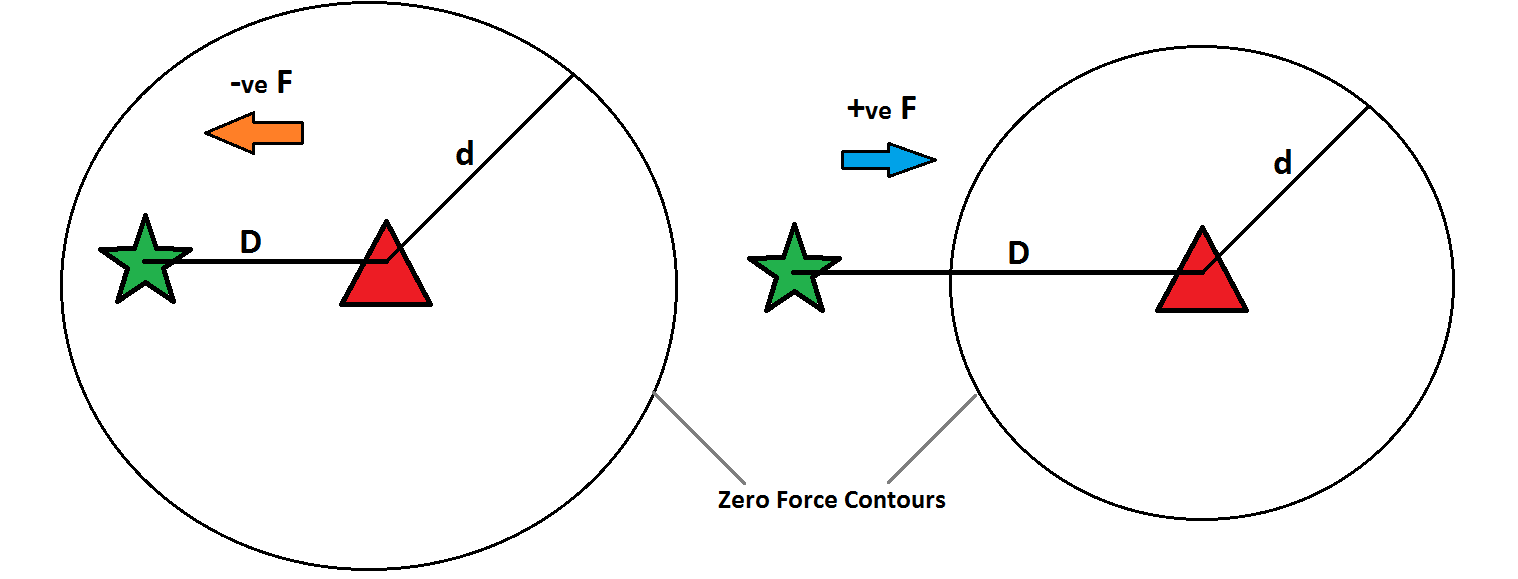
\includegraphics[width= 15cm]{mirror}
		\caption{The agent will attempt to move to the zero-potential force contour around the opponent. This is not a strict mirroring of the opponent, but rather allows the agent to move to optimal positions as opposed to just being guided by the opponent.}		
	\label{mirror}
\end{figure}

In general, the closer a tank is to the opponent, the higher the probability that it will hit the target. Thus, in order to improve the odds of our agent's firing solution, we would like the agent to be near the opponent. However, when trying to avoid being hit by incoming fire, we would like to be far from the opponent. In order to find a compromise we modeled $d$ as a function of the agent's health and the opponent's health. When the agent's health is higher, it moves closer to the opponent in order to maximize offensive capabilities. Else, the agent will move further away from the enemy to reduce the chance of being shot. Hence, the value of $d$ is determined as:
$$d = d_{const} - k_2*(\emph{Health}_{Agent} - \emph{Health}_{Opponent})$$
where $d_{const}$ is the minimum distance to maintain from the opponent, and $k_2$ provides regularization on how much to depend on the health difference.

\subsection*{Evasion Strategies}
When the opponent fires at the agent, the mirroring behavior is suppressed and an evasion strategy is chosen. At the moment, for training, we have designed the system to choose a random strategy. If we run enough training scenarios, we feel that the SVM will be able to find a good decision boundary with which to determine successful dodging strategies based on environmental properties. 

\subsubsection*{Dodge Left/Right}
In this strategy, the agent will move to the left or right of the opponent when it is fired upon. This movement strategy is represented in Figure \ref{LR}, where $\Psi$ is the relative bearing to the opponent ($-180^{\circ} \leq \Psi \leq 180^{\circ}$). There are two difference turning cases for $\Psi$: one when the agent is facing direction $d_1$ corresponding to bearing $\Psi_1$, and second when the agent is facing direction $d_2$ corresponding to bearing $\Psi_2$. Because we have a differential driven robot, we desire to turn a minimum distance to position our drive track perpendicular to the line of sight between us and the opponent. Achieving this angle is done in tandem with moving either forward or backward depending on whether we are dodging left or right. Dodging left / right are implemented separately, giving the agent the ability to choose each strategy.\\

\begin{figure}[h]
	\centering
		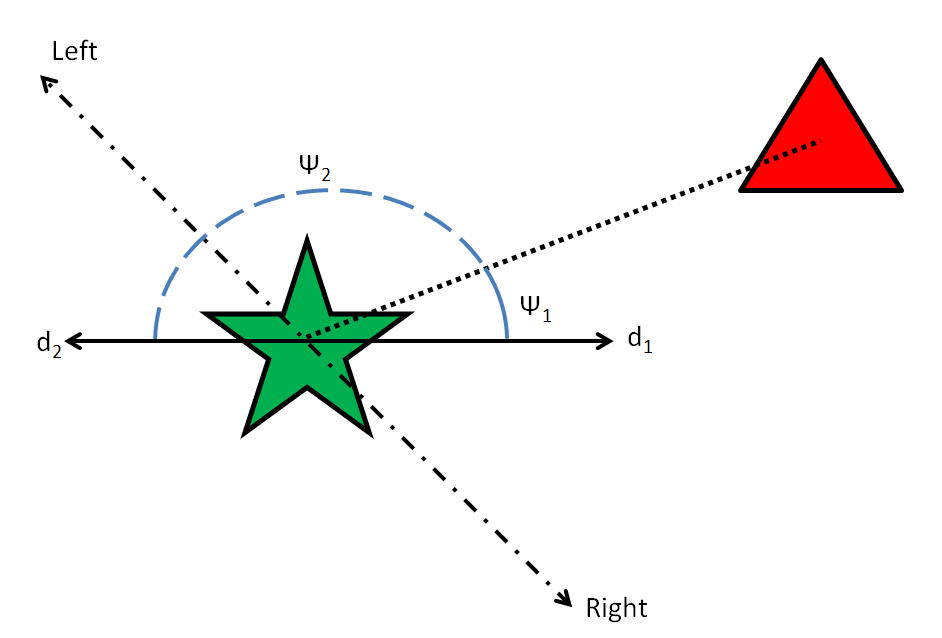
\includegraphics[width=7 cm]{LR}
	\caption{Left--Right dodging strategy. \emph{Note -- in Robocode, the angles are positive in a clockwise direction}}
	\label{LR}
\end{figure}

\subsubsection*{Feign}
In this strategy, upon detecting incoming fire, the agent immediately reverses its direction of motion. Robocode physics will require the agent to slow down to a stand still and then accelerate in the new direction. It is evident to us that this strategy will fail at closer distances and if the agent is moving directly towards or away from the opponent. Thus we expect the SVMs to discern this over time and only apply feign when it is optimal to do so.

\subsubsection*{Random Movement}
Random movement is useful against opponents that try to model their opponents. For this strategy, we set the turn control and forward movement control to a random value chosen from a uniform distribution. Agents that move in such a random manner are said to have flat movement profiles. They are hard to target, but certain advanced opponents are programmed to monitor such movement strategies when the agent approaches a wall or a corner, in which case the very nature of the environment will cause a spike in their movement profile. This kind of targeting is very specific to the opponent and we expect that our agent will learn that such behavior is not effective in certain regions of the environment.

\subsection*{Evaluation Methodology}
With these strategies created, we next needed a way to check the effectiveness of a evasion scheme. At its essence, we are testing the ability of the agent to stay alive, but we cannot rely on survival time as a measure of the effectiveness of a strategy. Thus, the effectiveness of the strategies are tested by the ability of the agent to dodge a particular shot fired at it. This is done through an estimate of the shot which is implemented using \emph{Bullet Tracking}

\subsubsection*{Bullet Tracking}
In order to determine if the evasion strategy employed was effective in dodging the bullet that was fired at the agent, we devised a way to track the bullet. In Robocode this is not a straight forward task, as the agent cannot sense a bullet using its radar. However, in order to fire a bullet, a tank must sacrifice some of its own energy. The radar-sensor can detect a drop in energy of the opponent, and using this we can determine if the enemy has fired a bullet as well as the bullet's velocity. This is given by the formula:
$$\emph{Bullet Velocity} = 20 - 3 * \emph{Energy Drop}$$
Using the velocity coupled with some basic Newtonian Physics\footnote{$\emph{Distance} = \emph{Velocity} * \emph{Time}$}, we can predict an equi-potential contour plot of how far away the bullet will be from the opponent's firing location at a given time step. The contours will be circular while resembling the motion of a wave. Hence, these estimates are known as \emph{waves}. Figure \ref{b_wave} illustrates this wave pattern taken on by bullets. Our objective is to see if we get hit by a bullet when the projected wave hits us, in which case we register a failure of the dodge strategy. Otherwise, we can conclude that we have successfully dodged the bullet.

\begin{figure}[h]
	\centering
		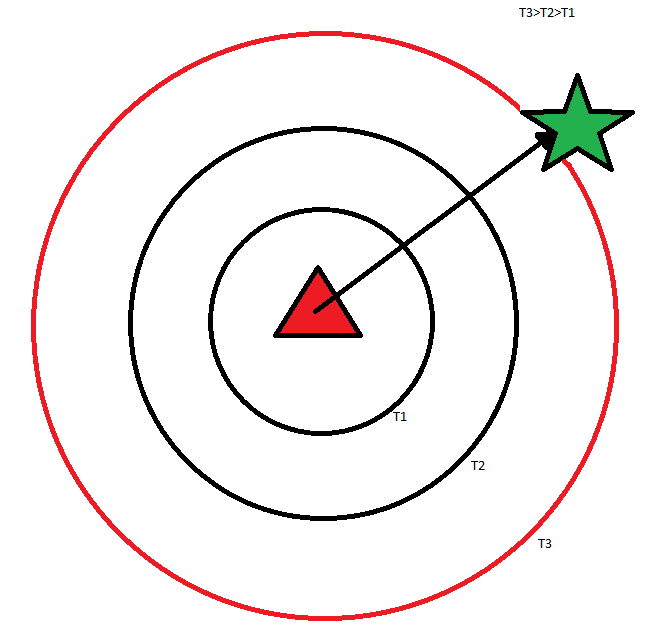
\includegraphics[width=7 cm]{bullet_wave.png}
	\caption{Bullet waves at different time steps}
	\label{b_wave}
\end{figure}

We are currently at a point where we can begin to collect data for evasive maneuvering. During the course of the training, we will look at the effectiveness of each strategy as the ability to dodge a particular shot while ignoring any other bullets which hit us during our evasive maneuver. We will collect data by running each evasion strategy multiple times against multiple different agents. 

\section{Future Milestones}
There will be five milestones to be completed before the project is finished: firstly, we will gather training data, train the SVMs,
and run tests for the evasion strategies. We will then repeat these processes while trying to reduce the number of features used. The next stage will be working on firing strategies. The last milestone is writing the
project report.

\subsection*{Gathering Training Data}
We recently finished designing an agent that randomly selects an evasion strategy when fired upon, and documents the features upon being fired upon. The next step is to gather training data on each evasion strategy using this agent against multiple agents. Every data point consists of a description of the battlefield at the time the bullet was fired, which evasion strategy was selected, and if the bullet hit or missed the robot.

{\bf Completion Date:}  03/16

\subsection*{Training SVMs}
With the training data from above, we will begin to train the SVMs for each evasion strategy, using the description of the battlefield as the features (with some manipulation to produce the true desired features), and hit/not hit as the classification labels. We plan on using libsvm, which has a Java plugin, as our SVM backend.

{\bf Completion Date:}   03/23

\subsection*{Testing}
Next, we will assess the performance of the system. We will modify our robot to look at the SVMs corresponding to each strategy every time a bullet is fired, and choose the best strategy in a way that maximizes the probability of not being hit. We will then compare the performance of this implementation versus randomly choosing a strategy.

{\bf Completion Date:}  03/30

\subsection*{Feature Space Reduction}
In order to minimize the complexity of the model, and to possibly increase the performance by avoiding over-fitting, we will try to reduce the number of features used to describe the battlefield. In order to do so, we will train and test the robot with different combinations of features, keeping track of how the performance is affected. 

{\bf Completion Date:}  04/06

\subsection*{Offensive Strategies}
Having learned good evasion tactics, we will then focus on the offensive strategies. We have decided to leave the details of how we will handle this intentionally vague. We hope to to learn from our experience with the evasive strategies in order to build upon them when implementing our targeting scheme. 

{\bf Completion Date:}  04/20

\subsection*{Final Report}
The final report is due on 04/24.

\section{Conclusion}

Thus far, we have successfully written an agent capable of implementing the previously discussed evasion techniques when fired upon by an opposing agent. This agent is also capable of continuously tracking the enemy, as well as the bullets fired from the enemy, in an effort to capture the data needed to train each evasion strategy's SVM. We are currently in the process of choosing the exact features desired from the environment upon each evasion attempt, and will then begin collecting data with which to train the SVMs on. After such training, we will then be able to evaluate the evasion system in an effort to maximize the agent's ability to evade bullets as well as to capture those features most important to understanding the best strategy given each unique situation. Lastly, we will move onto repeating these steps, with the additional knowledge gained throughout our experience, to design an effective targeting and firing system. At the end of this project, we will have novelly employed machine learning techniques to artificial intelligence agents in order to improve their ability to make decision informed by their perceptual knowledge of the environment.

\bibliographystyle{IEEEtranS}
\bibliography{sources}

\end{document}


\def\therefore{\boldsymbol{\text{ }
\leavevmode
\lower0.4ex\hbox{$\cdot$}
\kern-.5em\raise0.7ex\hbox{$\cdot$}
\kern-0.55em\lower0.4ex\hbox{$\cdot$}
\thinspace\text{ }}}
